\begin{tikzpicture}[x=1pt,y=1pt,
    every node/.style={font=\footnotesize},
    ah/.style={draw opacity=0,line width=0.08,fill opacity=1},
    lbl/.style={fill=white,align=center,inner sep=2.5pt,line width=0.6pt},
    dim/.style={fill=white,align=center,inner sep=2pt,draw=none,font=\scriptsize},
    reg/.style={line width=1.2pt}]

% ---- Photograph -------------------------------------------------------
\node [anchor=south west,inner sep=0] at (0,0)
  {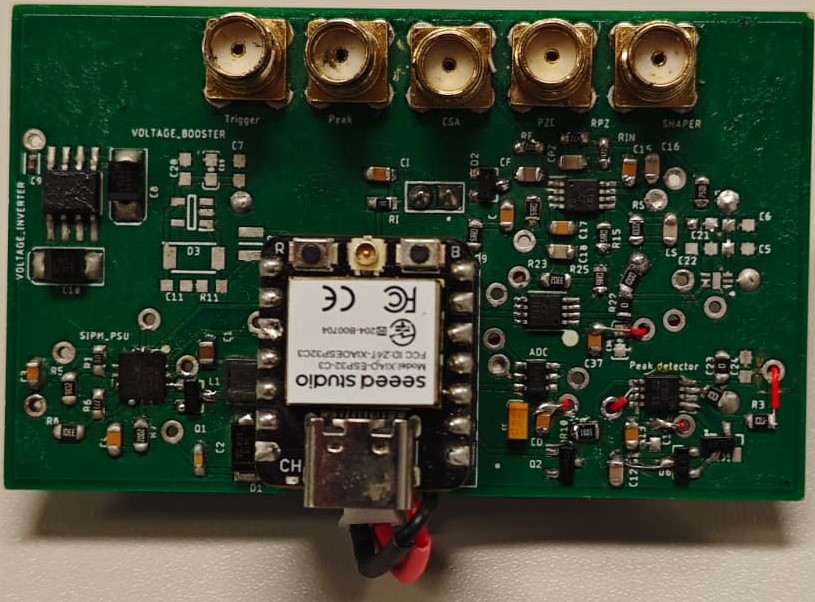
\includegraphics[width=186pt,height=127pt]{images/pcb_teste.jpg}};

% ---- Region outlines ---------------------------------------------------
\draw [reg,color={rgb, 255:red, 241; green, 74; blue, 64 }]
      (2.55,24.84) rectangle (52.93,59.98);                 % SiPM power supply
\draw [reg,color={rgb, 255:red, 26; green, 111; blue, 223 }]
      (116.09,72.67) rectangle (166.47,101.07);             % pulse shaping
\draw [reg,color={rgb, 255:red, 204; green, 153; blue, 0 }]
      (113.63,34.27) rectangle (129.67,53.47);              % ADC
\draw [reg,color={rgb, 255:red, 55; green, 173; blue, 107 }]
      (113.51,63.72) .. controls (118.22,73.60) and (139.09,68.88) .. (153.45,57.88)
   .. controls (167.81,46.87) and (177.68,49.12) .. (178.35,43.95)
   .. controls (179.03,38.79) and (182.39,38.56) .. (172.97,30.48)
   .. controls (163.55,22.40) and (163.98,22.18) .. (151.65,21.95)
   .. controls (139.33,21.72) and (126.97,19.26) .. (126.86,25.54)
   .. controls (126.74,31.83) and (140.14,43.95) .. (136.62,50.01)
   .. controls (133.10,56.08) and (108.80,53.84) .. (113.51,63.72) -- cycle ;

% ---- Labels over the board (no arrows) --------------------------------
\node [lbl,draw=none,font=\scriptsize,anchor=center] at (83.33,54.66) {MCU};
\node [lbl,draw={rgb, 255:red, 204; green, 153; blue, 0 },
       font=\scriptsize,anchor=center] at (114.30,27.04) {ADC};
\node [lbl,draw={rgb, 255:red, 241; green, 74; blue, 64 },anchor=center]
      at (27.90,13.25) {SiPM\\Power Supply};
\node [lbl,draw={rgb, 255:red, 55; green, 173; blue, 107 },anchor=center]
      at (163,13.25) {Pulse\\Discrimination};

% ---- Pulse shaping (right of the board) -------------------------------
\node [lbl,draw={rgb, 255:red, 26; green, 111; blue, 223 },anchor=west]
      at (165,86.90) {Pulse\\Shaping};



% ---- Signal test points (only arrow in the figure) --------------------
\node [lbl,draw={rgb, 255:red, 81; green, 81; blue, 81 },anchor=center]
      at (27.60,88) {Signal\\Test Points};
\draw [color={rgb, 255:red, 81; green, 81; blue, 81 },line width=1.1pt] (50,99) -- (50,108);
\draw [shift={(50,116)},rotate=270,ah,fill={rgb, 255:red, 81; green, 81; blue, 81 }]
      (7.85,-3.78) -- (0,0) -- (7.85,3.78) -- cycle ;

% ---- Width dimension (7 cm) --------------------------------------------
\draw [line width=1.1pt,black] (3.56,134) -- (184.42,134);
\draw [shift={(3.56,134)},rotate=0,ah,fill=black]
      (7.85,-3.78) -- (0,0) -- (7.85,3.78) -- cycle ;
\draw [shift={(184.42,134)},rotate=180,ah,fill=black]
      (7.85,-3.78) -- (0,0) -- (7.85,3.78) -- cycle ;
\node [dim,anchor=center] at (94,134) {7~cm};

% ---- Height dimension (4.3 cm) -----------------------------------------
\draw [line width=1.1pt,black] (-8,23.50) -- (-8,125.65);
\draw [shift={(-8,23.50)},rotate=90,ah,fill=black]
      (7.85,-3.78) -- (0,0) -- (7.85,3.78) -- cycle ;
\draw [shift={(-8,125.65)},rotate=270,ah,fill=black]
      (7.85,-3.78) -- (0,0) -- (7.85,3.78) -- cycle ;
\node [dim,anchor=center,rotate=90] at (-8,74.60) {4.3~cm};

\end{tikzpicture}